\section{Results}
To demonstrate \deploy's capability conduct transition
scenario analysis effectively and meet the objectives described in section 
\ref{sec:obj}, this section 
(1) demonstrates \deploy's capability in simple transition scenarios, 
(2) compares the use of different prediction methods in  EG01-EG23, EG01-EG24, 
EG01-EG29, and EG01-EG30 transition scenarios, and
(3) demonstrates successful \deploy setup of EG01-EG23, EG01-EG24, 
EG01-EG29, and EG01-EG30 transition scenarios. 
The input files and scripts to reproduce the results and plots in this
paper are found in \cite{noauthor_arfc/d3ploy:_2019} and 
\cite{chee_arfc/transition-scenarios_2018}. 

\subsection{Demonstration of \deploy's capabilities}
\label{sec:demo}
We conducted a simple transition scenario simulation with
linearly increasing power demand
to demonstrate \deploy's capabilities and inform input parameter 
choices when setting up complex many-facility transition scenarios. 
This simulation only includes
three facility types: \texttt{source}, \texttt{reactor}, and 
\texttt{sink}. 
The simulation begins with ten \texttt{reactor} facilities 
(\texttt{reactor1} to \texttt{reactor10}). 
These reactors have staggered cycle lengths and lifetimes to prevent 
simultaneous refueling and setup gradual decommissioning. 
\deploy deploys \texttt{new reactor} facilities
to fill power supply gap created when the initial \texttt{reactor} 
facilities decommision. 
Table \ref{tab:demonstrations} shows the \deploy input parameters 
for this simulation.  

    \begin{table}[]
        \caption{\deploy's input parameters for the simple transition 
        scenario with linearly increasing power demand.}
        \label{tab:demonstrations}
        \begin{tabular}{l|ll}
        \hline
                                  & \textbf{Input Parameters}          & \textbf{Simple Transition Scenario} \\ \hline
        \multirow{5}{*}{\textbf{Required}} & Demand driving commodity  & \multicolumn{1}{l}{Power}                            \\
                                  & Demand equation [MW]          &  $t<40 = 1000, t\geq 40 = 1000+250t$                                                    \\
                                  & Available facilities    &  \texttt{Source}, \texttt{Reactor}, \texttt{Sink}                                                    \\
                                  & Prediction method         &  \texttt{FFT}                                                    \\
                                  & Deployment driving method & \multicolumn{1}{l}{Installed Capacity}               \\ \hline
        \multirow{2}{*}{\textbf{Optional}} & Buffer type               & \multicolumn{1}{l}{Absolute}                         \\
                                  & Buffer size               &  Power: 2000MW, Fuel: 1000kg                                                    \\ \hline
        \end{tabular}%
        \end{table}

Figures \ref{fig:growingtransition-power}, \ref{fig:growingtransition-fuel},
and \ref{fig:growingtransition-spentfuel} demonstrate \deploy's capability 
to deploy reactor and supporting facilities to minimize undersupply 
when meeting linearly increasing power demand and subsequent secondary 
commodities demand. 
In Figure \ref{fig:growingtransition-power} there exists no time steps 
in which the supply of power falls under demand, meeting the main 
objective of \deploy. 
By using a combination of the \texttt{FFT} method for 
predicting demand and a power supply buffer of 2000MW 
(the capacity of 2 reactors), we minimized the number of 
undersupplied time steps for every commodity.

In figure \ref{fig:growingtransition-fuel},
a large-throughput source facility is initially
deployed to meet the large initial fuel demand for the commissioning 
of ten reactors. 
By having a large-throughput source facility exist for the 
first few time steps, \deploy does not deploy supporting
facilities that become redundant at later times in  
the simulation.
This reflects reality in which reactor manufacturers accumulate
an appropriate amount of fuel inventory before starting 
up reactors. 
There is one time step in which a power undersupply exists after the 
decommissioning of the large initial facility; 
this is unavoidable as the prediction methods in \deploy are 
unable to foresee this sudden drop in demand. 

\begin{figure}[]
    \centering
    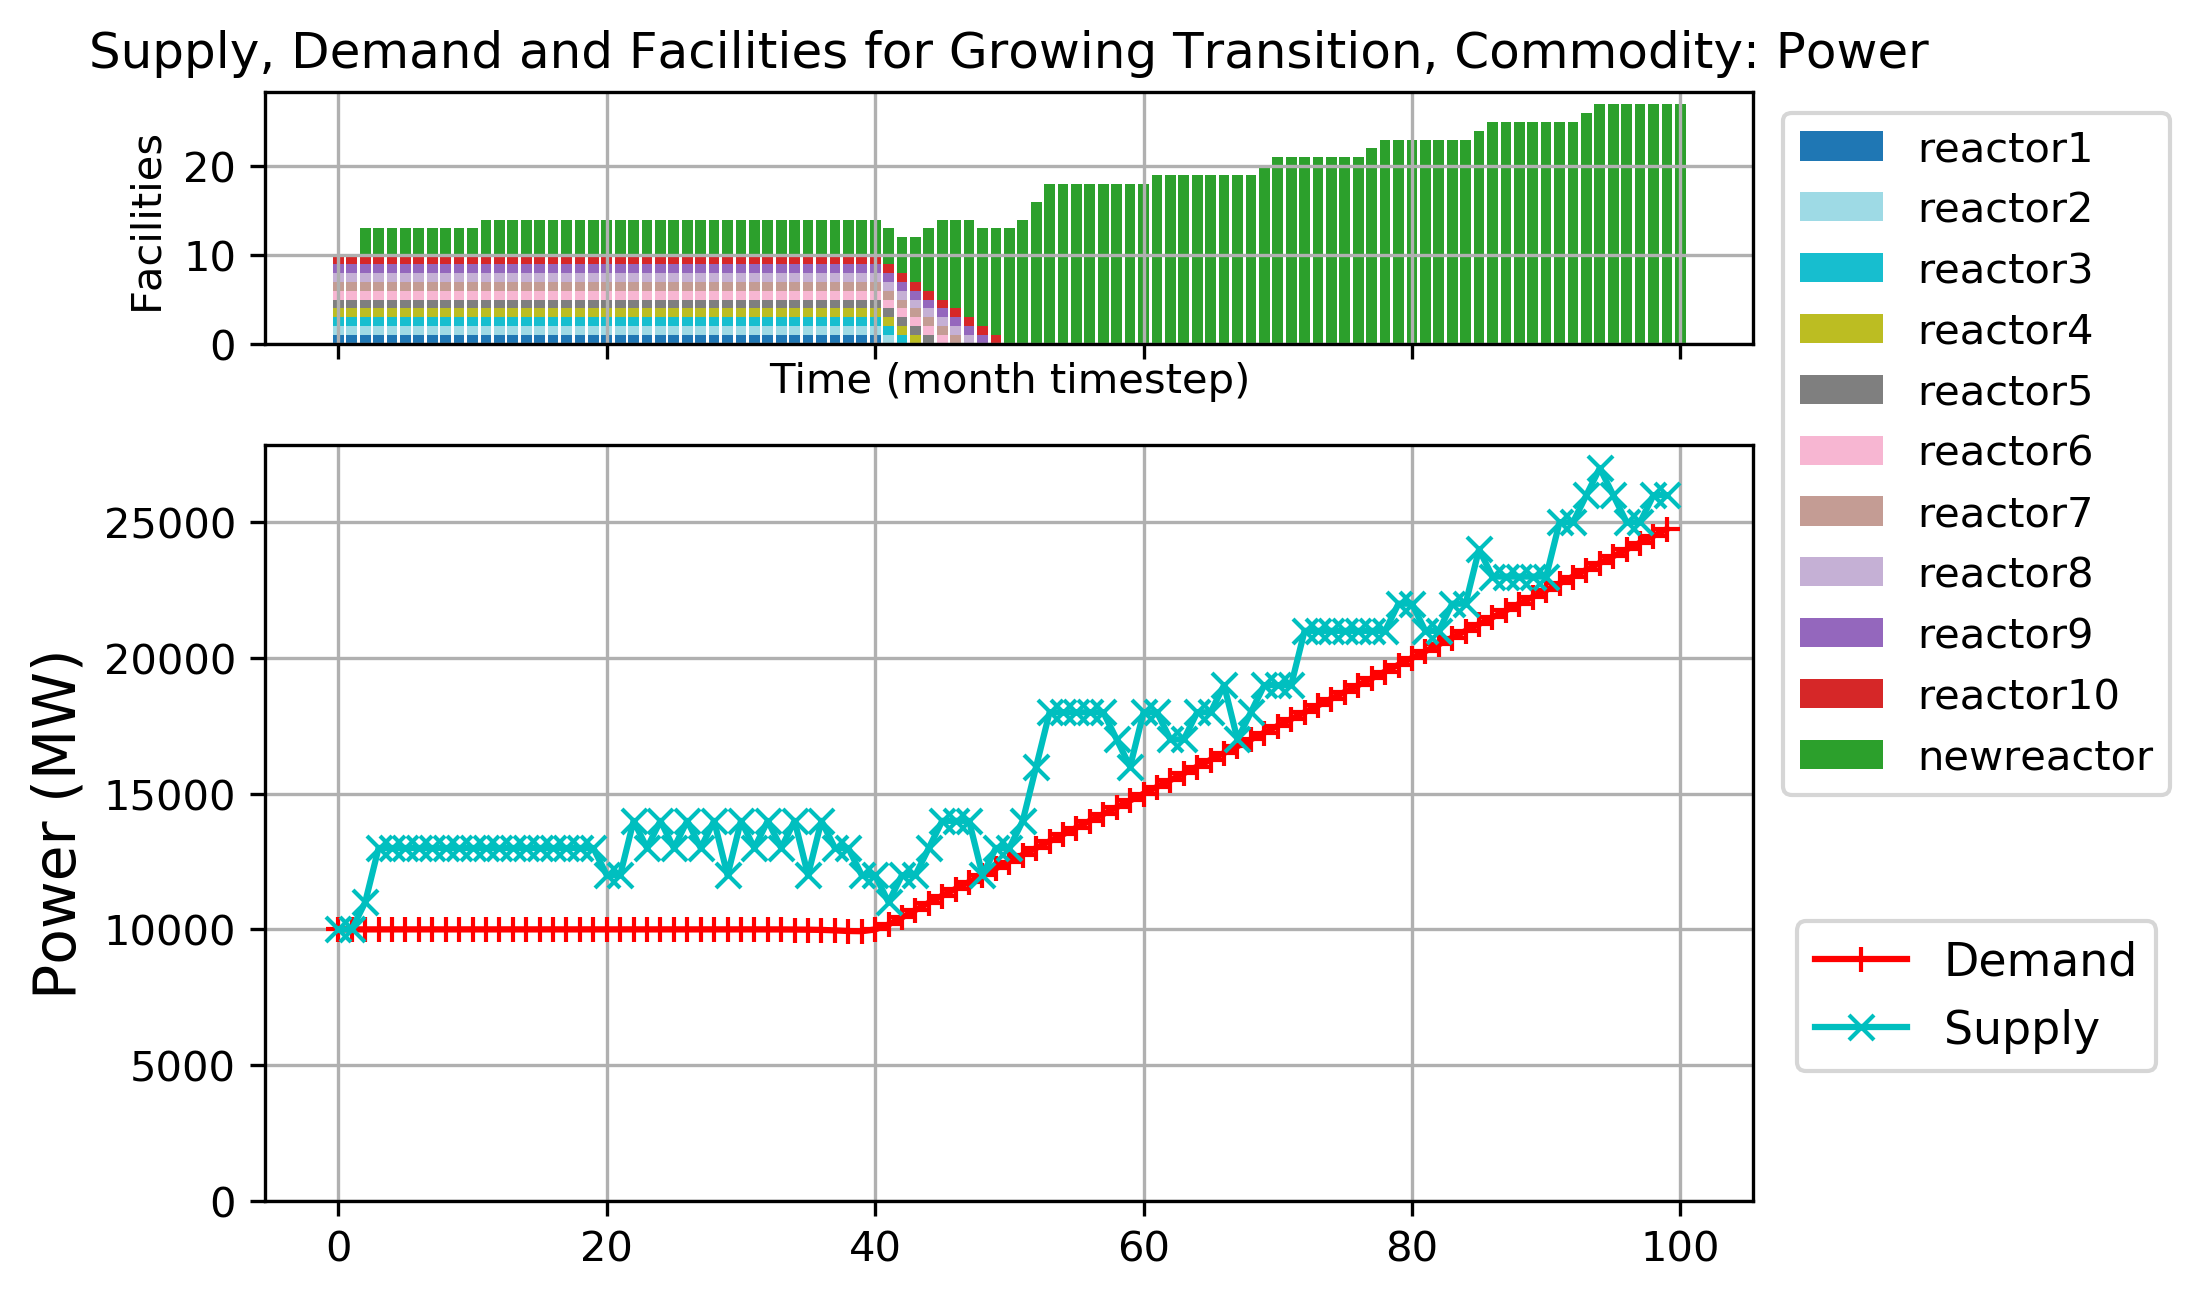
\includegraphics[width=\linewidth]{figures/growingtransition-power.png} 
        \caption{Power demand and supply, and reactor facility deployment plot for  
        a simple linearly increasing power demand transition scenario with 
        three facility types: \texttt{source}, \texttt{reactor}, and \texttt{sink}.
        Power demand is a user-defined equation and power is supplied by the reactors.
        There are no time steps with undersupply of power.}
        \label{fig:growingtransition-power}
\end{figure}

\begin{figure}[]
    \centering
    \begin{subfigure}[t]{1\textwidth}
        \centering
        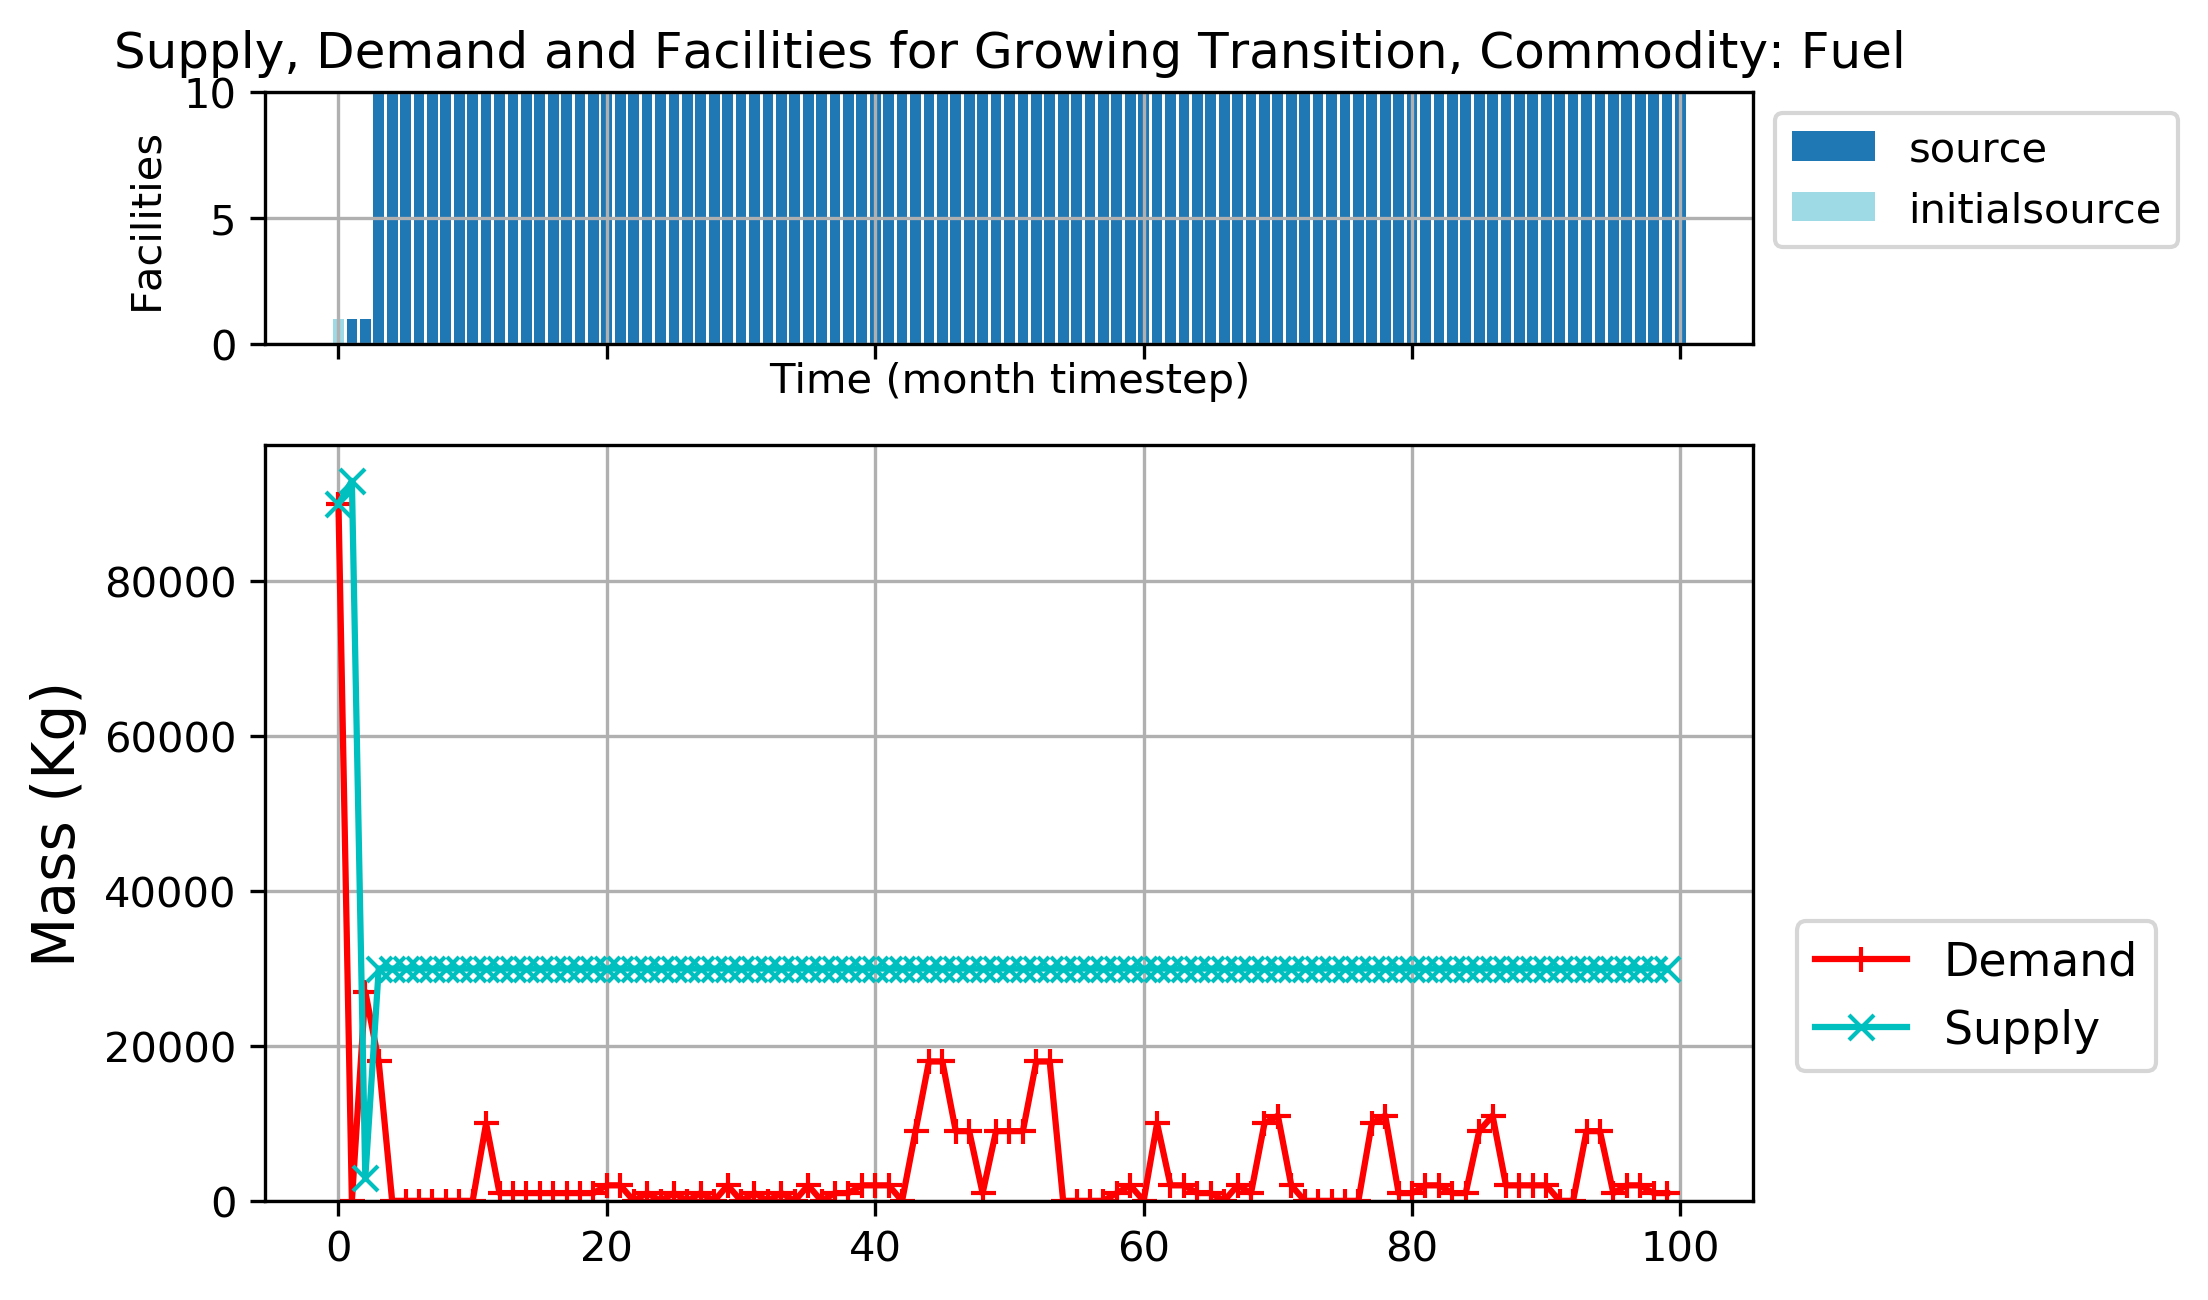
\includegraphics[width=\linewidth]{figures/growingtransition-fuel.png} 
        \caption{Fuel demand and supply, and source facility deployment plot.
        Fuel is demanded by reactors and supplied by source facilities.
        There is only one time step with undersupply of fuel.}
	    \label{fig:growingtransition-fuel}
    \end{subfigure}
    \begin{subfigure}[t]{1\textwidth}
        \centering
        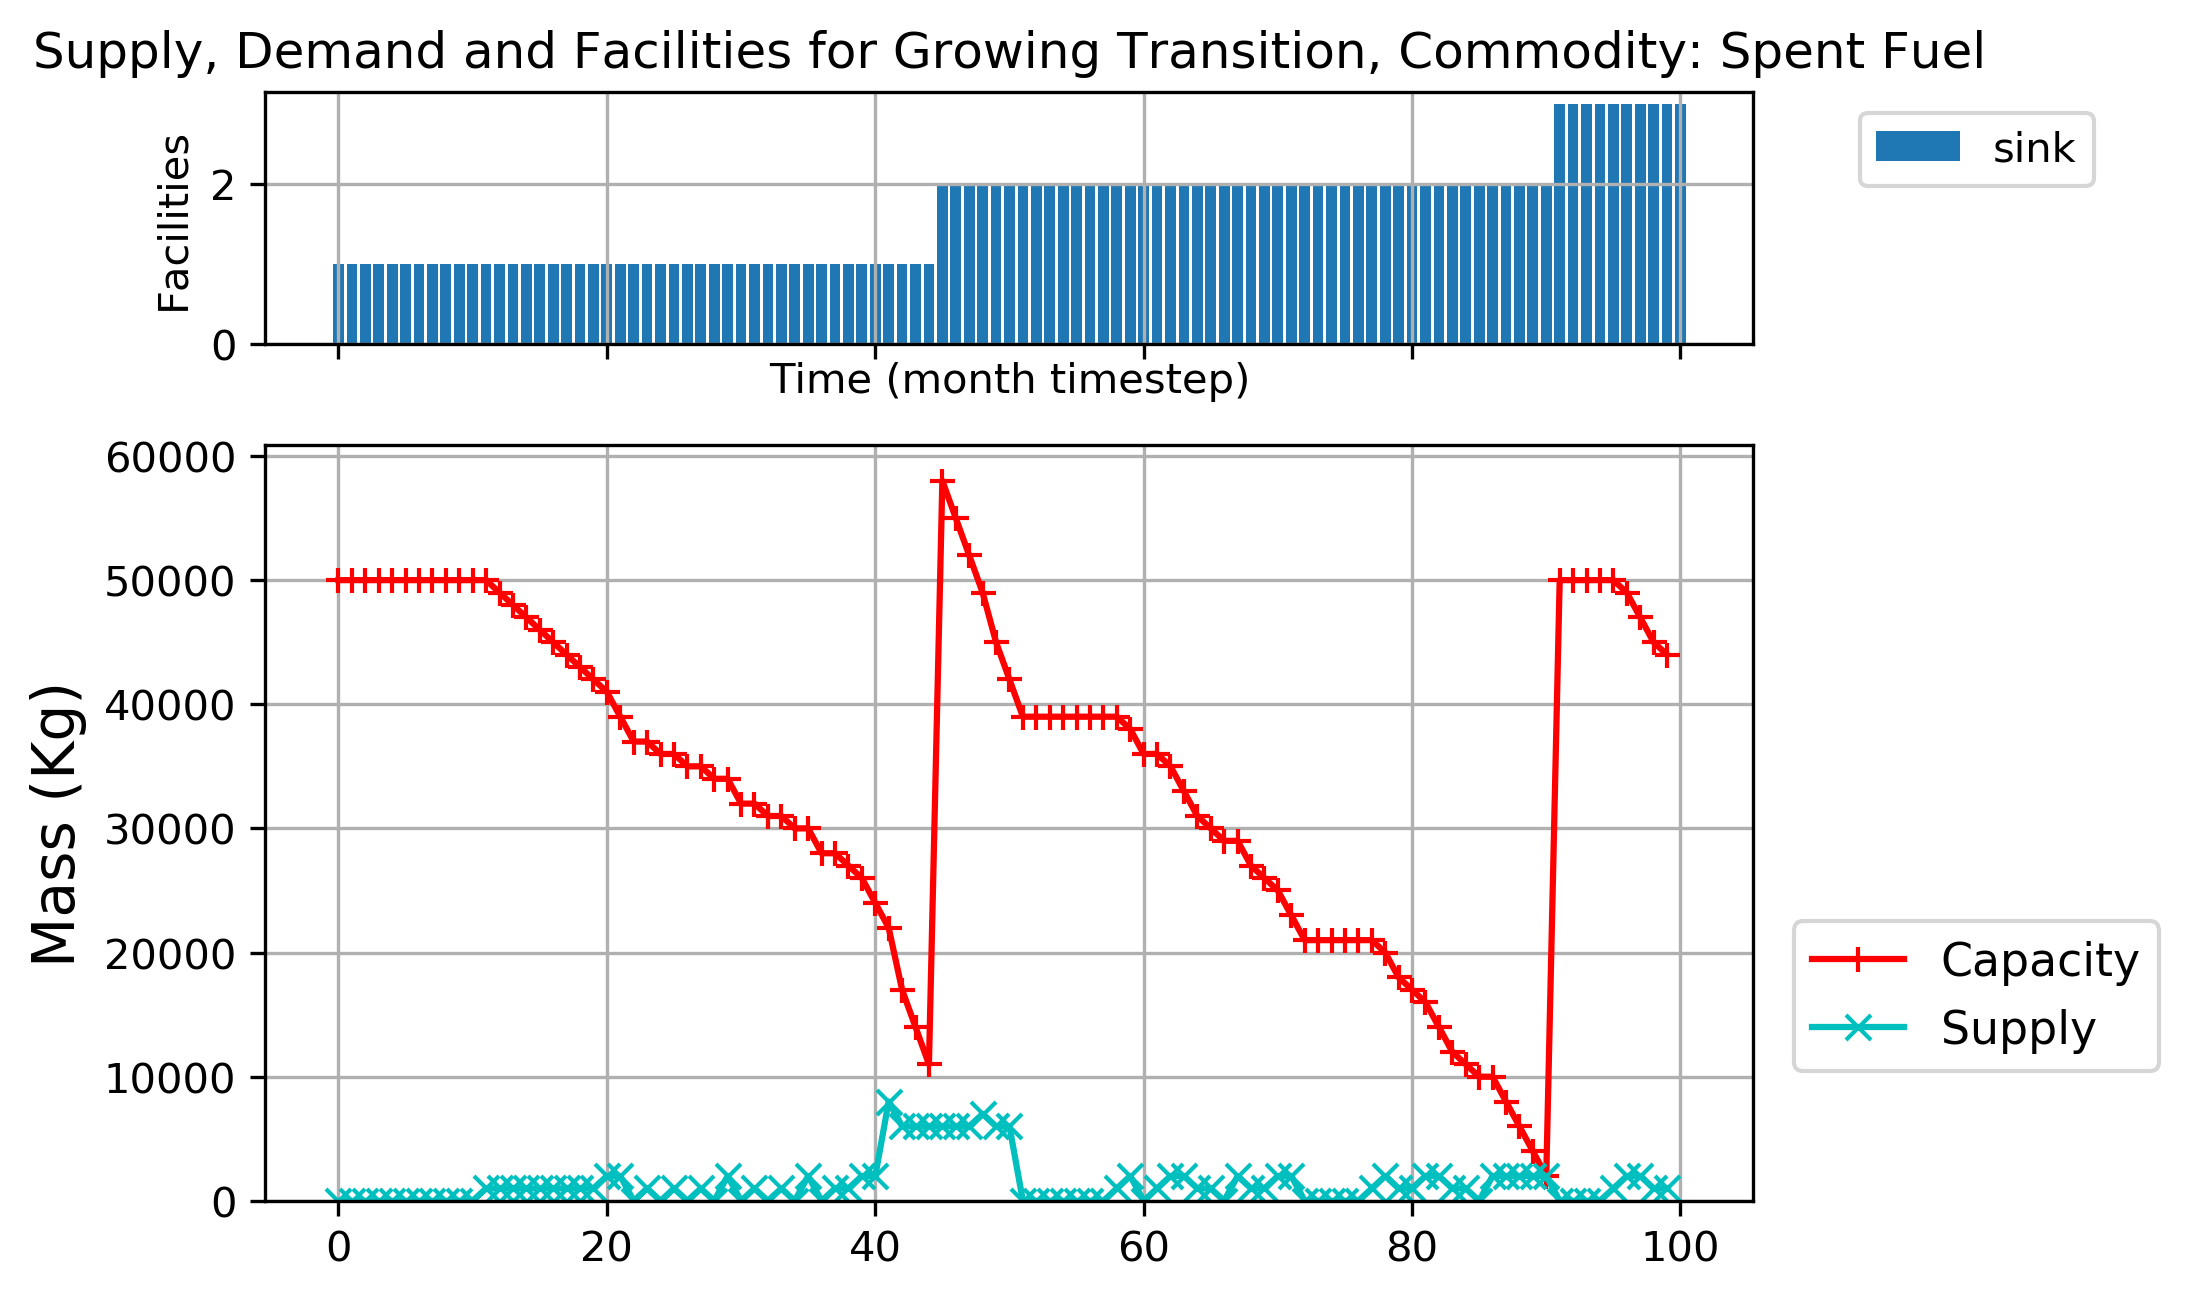
\includegraphics[width=\linewidth]{figures/growingtransition-spentfuel.png} 
        \caption{Spent fuel demand and supply, and sink facility deployment plot.
            Spent Fuel is supplied by reactors and the capacity to store them 
            is provided by sink facilities.
        There are no time steps with under-capacity of sink space.}
        \label{fig:growingtransition-spentfuel}
    \end{subfigure}
    \caption{Simple linearly increasing power demand transition scenario with 
    three facility types: \texttt{source}, \texttt{reactor}, and \texttt{sink}.}
\end{figure}
